\ifdefined\COMPLETE
\else
    \input{./preambule_Analyse_binaire.ltx}
    \begin{document}
\fi

\chapter{L'analyse binaire}

\section{Ensembles binaires algébriques}

On appelle variable ou fonction binaire, toute variable ou toute fonction
ne pouvant prendre que l'une des deux \textit{valeurs algébrique distinctes
$a\neq b$}, à l'exclusion de toute autre.

L'\textit{ensemble} «  $E_{ab}$  » des variables et des fonctions
ainsi définies est appelé {ensemble binaire algébrique}.

Le choix de l'ensemble binaire $E_{01}$ se justifie par l'adoption
d'une valeur d'absorption « $0$ » et d'une valeur neutre « $1$ » qui
font du \textit{produit algébrique} une fonction binaire appartenant
au même ensemble .

\subsection{Produit}

Soient $n$ fonctions binaires $f_{1},f_{2},\ldots f_{n}$ telles
que $f_{i}\in E_{01},\forall i=1,2,\ldots n$, le produit algébrique
de ces $n$ fonctions appartient à l'ensemble $E_{01}$.

\centerline{$(P=f_{1}.f_{2}\ldots f_{n})\in E_{01}$}

Le produit $P$ est en effet égal à l'unité lorsque toutes les fonctions
en facteur sont simultanément égales à l'unité. $(f_{1}=f_{2}=\ldots=f_{n}=1)\Longleftrightarrow(P=1)$.

Il est nul dans tous les autres cas.

Nous appellerons également le produit « $P$ » fonction « ET » quand
il fera l'objet d'ap\-pli\-ca\-tion technologiques.

\bigskip 

\begin{figure}[htb]
\begin{centering}

\includegraphics[width=4cm]{Figures/ET} \vspace{1cm}
\par\end{centering}
\caption{Fonction « ET » ~\textendash{} \textbf{produit} $a.b.c=Y$}
\label{fig:ET} 
\end{figure}


\newpage 

\subsection{Produel}

Il faut choisir un symbolisme simple qui puisse traduire dans l'expression
écrite, la dualité qui caractérise les ensembles binaires et qui permette,
en utilisant si possible les deux dimensions du plan, l'établissement
de relations duales élémentaires.

Nous savons aussi, par dualité, qu'il est possible de faire correspondre
au produit, la \textit{fonction algébrique binaire} :

\centerline{$\pi=1-P$} \centerline{$\pi=1-(1-f_{1}).(1-f_{2})\ldots(1-f_{n})=\overline{f_{1}.f_{2}\ldots f_{n}}$}
\centerline{$f_{i}\in E_{01},\forall i=1,2,\ldots n)\Longrightarrow(\pi\in E_{01})$}

La fonction $\pi$ est égale à zéro lorsque toutes les fonction $f_{i}$
sont simultanément nulles,

\centerline{$f_{1}=f_{2}=\ldots=f_{n}=0)\Longrightarrow(\pi=0)$}

et qu'elle est égale à l'unité dans tous les autres cas, puisqu'il
suffit qu'une fonction $f_{i}$ au moins soit égale à l'unité pour
que le produit algébrique $(1-f_{1}).(1-f_{2})\ldots(1-f_{n})$ soit
nul ; ce qui entraîne $\pi=1$.

Nous conviendrons alors de représenter la fonction « $\pi$ » ~,
que nous appellerons « \textit{produel} » ~\footnote{Les racines latines « pro » et « duales » ont été choisies
dans la constitution du né\-o\-lo\-gisme « pro\-duel » pour
marquer d'une part la nécessité de conserver la dualité dans les expressions
binaires et aussi par analogie avec le mot « produit » ~.} en groupant les termes qui la composent suivant une colonne verticale
par analogie avec l'écriture horizontale du produit, pour traduire
dans le symbolisme, la propriété de dualité.

\begin{center}
$\pi=\begin{array}{|c|}
f_{1}\\
f_{2}\\
\vdots\\
f_{n}
\end{array}=1-(1-f_{1}).(1-f_{2})\ldots(1-f_{n})=\overline{f_{1}.f_{2}\ldots F_{n}}$
\end{center}

Nous appellerons également « $\pi$ » ~, fonction « OU »  dans
le cas des applications technologiques.

\begin{figure}[htb]
\center{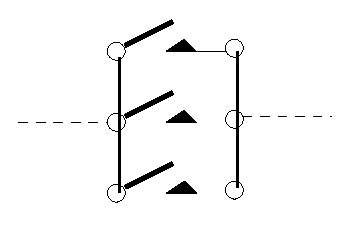
\includegraphics[width=4cm]{Figures/OU}} \vspace{1cm}

\setbox1=\hbox{$\begin{array}{r|c|l}
 & a\\
\text{Fonction «  OU » {\bf produel} : }  & b & =1-(1-a).(1-b).(1-c)=Z\\
 & c
\end{array}$} 

\caption{\box1}

\label{fig:OU} 
\end{figure}

\subsection{Définition d'une \emph{structure logique binaire}}

La structure logique binaire se caractérise essentiellement par les
deux opérations fondamentales qui ont des propriétés réciproques.
Les symboles peuvent représenter des ensembles, des partitions d'ensembles,
des groupes, des classes ou des éléments, voire même des opérateurs.

Les deux opérations sont, à la fois, \textbf{commutatives, associatives,
réciproquement distributives} et possèdent, toutes deux, \textbf{la
propriété d'idempotence} ; ce qui permet d'écrire successivement les
égalités suivantes~:

\begin{center}
{\scriptsize{}}%
\begin{tabular}{|l|l|}
\hline 
\multicolumn{1}{|c|}{\textit{\scriptsize{}Produit}} & \multicolumn{1}{|c|}{\textit{\scriptsize{}Produel}}\tabularnewline
\hline 
 & \tabularnewline
{\scriptsize{}$P=a.b.c$ } & {\scriptsize{}$\begin{array}{rcl}
\pi & = & \begin{array}{|c|}
a\\
b\\
c
\end{array}\\
 & = & 1-(1-a).(1-b).(1-c)
\end{array}$ }\tabularnewline
{\scriptsize{}\textendash{} élément neutre « 1 » ~} & {\scriptsize{}\textendash{} élément neutre « 0 » ~}\tabularnewline
\multicolumn{1}{|c|}{{\scriptsize{}$(1.f)=f$}} & \multicolumn{1}{|c|}{{\scriptsize{}$\begin{array}{|c|}
0\\
f
\end{array}=f$}}\tabularnewline
{\scriptsize{}\textendash{} élément absorbant « 0 » ~} & {\scriptsize{}\textendash{} élément absorbant « 1 » ~}\tabularnewline
\multicolumn{1}{|c|}{{\scriptsize{}$(0.f)=0$}} & \multicolumn{1}{|c|}{{\scriptsize{}$\begin{array}{|c|}
1\\
f
\end{array}=1$}}\tabularnewline
{\scriptsize{}\textendash{} commutatif : $\begin{array}{|c|}
ab\end{array}=\begin{array}{|c|}
ba\end{array}$ } & {\scriptsize{}\textendash{} commutatif : $\begin{array}{|c|}
a\\
b
\end{array}=\begin{array}{|c|}
b\\
a
\end{array}$ }\tabularnewline
{\scriptsize{}\textendash{} associatif : $\begin{array}{|c|c||}
a & bc\end{array}=\begin{array}{||c|c|}
ba & c\end{array}=\begin{array}{|c|}
cba\end{array}$ } & {\scriptsize{}\textendash{} associatif : $\begin{array}{||c||}
\multicolumn{1}{|c|}{a}\\
b\\
c
\end{array}=\begin{array}{||c||}
b\\
a\\
\multicolumn{1}{|c|}{c}
\end{array}=\begin{array}{|c|}
c\\
b\\
a
\end{array}$ }\tabularnewline
 & {\scriptsize{}\textendash distributif : }\tabularnewline
{\scriptsize{}\textendash{} distributif : $\begin{array}{|c|}
ab\\
ac\\
d
\end{array}=\begin{array}{|c|}
a\;\begin{array}{|c}
b\\
c
\end{array}\\
d
\end{array}=\begin{array}{|c|}
d\\
\begin{array}{c|}
b\\
c
\end{array}\;a
\end{array}=\begin{array}{|c|}
d\\
b\\
c
\end{array}\begin{array}{c|}
d\\
a
\end{array}$ } & {\scriptsize{}$\begin{array}{|c|c|}
a & a\\
b & c
\end{array}\begin{array}{c|}
d\end{array}=\begin{array}{|c|}
a\\
bc
\end{array}=\begin{array}{|c}
d\end{array}\begin{array}{|c|}
bc\\
a
\end{array}=\begin{array}{|c|}
dbc\\
da
\end{array}$}\tabularnewline
{\scriptsize{}\textendash{} idempotent : $\begin{array}{|c|}
aa\ldots a\end{array}=\begin{array}{|c|}
a\end{array}$ } & {\scriptsize{}\textendash{} idempotent : $\begin{array}{|c|}
a\\
a\\
\vdots\\
a
\end{array}=\begin{array}{|c|}
a\end{array}$ }\tabularnewline
\multicolumn{1}{|c|}{{\scriptsize{}$P=\overbrace{a.a\ldots a}^{n}=a^{n}$}} & \multicolumn{1}{|c|}{{\scriptsize{}$\pi=\left.\begin{array}{|c|}
a\\
a\\
\vdots\\
a
\end{array}\right\} n=1-(1-n)^{n}$}}\tabularnewline
\multicolumn{1}{|c|}{{\scriptsize{}pour $a=0\hfil(0)^{n}=0$}} & \multicolumn{1}{|c|}{{\scriptsize{}pour $a=0\hfil\pi=1-(1)^{n}=0$}}\tabularnewline
\multicolumn{1}{|c|}{{\scriptsize{}pour $a=1\hfil(1)^{n}=1$}} & \multicolumn{1}{|c|}{{\scriptsize{}pour $a=1\hfil\pi=1-(1)^{n}=1$}}\tabularnewline
\multicolumn{1}{|l|}{{\scriptsize{} }%
\begin{minipage}[t]{7.5cm}%
{\scriptsize{} Si dans un produit, deux facteurs sont complémentaires,
le produit est nul. }%
\end{minipage}} & \multicolumn{1}{|l|}{{\scriptsize{} }%
\begin{minipage}[t]{6cm}%
{\scriptsize{} Si dans un produel, deux facteurs duals sont complémentaires,
le produel est égal à l'unité }%
\end{minipage}}\tabularnewline
{\scriptsize{}$P=f.\overline{f}.P_{1}$ } & {\scriptsize{}$\pi=\begin{array}{|c|}
f\\
\overline{f}\\
\pi_{1}
\end{array}=1-(1-f).f.(1-\pi_{1})$ }\tabularnewline
{\scriptsize{}$P=f.(1-f)P_{1}=(f-f^{2}).P_{1}$ } & {\scriptsize{}$=1-(f-f^{2}).(1-\pi_{1}=1-0.(1-\pi_{1})$ }\tabularnewline
{\scriptsize{}$P=(0.P_{1})=0$ } & {\scriptsize{}$\pi=\begin{array}{|c|}
1\\
\pi_{1}
\end{array}=1$ }\tabularnewline
{\scriptsize{}$(f.\overline{f})=0$ } & {\scriptsize{}$\begin{array}{|c|}
f\\
\overline{f}
\end{array}=1$ }\tabularnewline
\hline 
\end{tabular} 
\end{center}

\subsection{Théorème de De Morgan}

Ce théorème est contenu implicitement dans les définitions précédentes.

\begin{center}
$1-\begin{array}{|c|}
f_{1}\\
f_{2}\\
\vdots\\
f_{n}
\end{array}=\overline{\begin{array}{|c|}
f_{1}\\
f_{2}\\
\vdots\\
f_{n}
\end{array}}=\overline{f_{1}}.\overline{f_{2}}\ldots\overline{f_{n}}=(1-f_{1}).(1-f_{2})\ldots(1-f_{n})$
\end{center}

\textit{Le complément d'un produel est égal au produit des compléments
des facteurs duals qui le composent.}

\begin{center}
$\overline{f_{1}.f_{2}\ldots f_{n}}s=\begin{array}{|c|}
\overline{f_{1}}\\
\overline{f_{2}}\\
\vdots\\
\overline{f_{1}}
\end{array}=1-(f_{1}.f_{2}\ldots f_{n})$
\end{center}

\textit{Le complément d'un produit est égal au produel des compléments
des facteurs qui le composent}.

\subsection{Fonctions canoniques et tables de vérité}

Toute fonction binaire peut s'exprimer soit par un produit de produels
soit par un produel de produits. Les expressions obtenues sont appelées
« \textit{fonctions canoniques} » ~.

Si une fonction binaire dépend de « $n$ » variables distinctes
$x_{1},x_{2},\ldots x_{n}$, nous ne pouvons envisager au total que
$2^{n}$ combinaisons de valeurs distinctes (0 ou 1) de ces « $n$ » variables.
Si la fonction binaire est égale à l'unité pour « $p$ »  combinaisons,
elle est nécessairement ????????????????

Nous appellerons « \textit{ transposition}  » \label{transposition}~,
\textit{le passage, pour une même fonction, de la première à la deuxième
forme canonique et réciproquement}.

\subsubsection{Établissement de la première forme canonique}

On inscrit horizontalement les variables dans un ordre quelconque,
puis on porte successivement sous ces variables dans le sens horizontal,
les combinaisons de valeurs pour lesquelles la fonction est égale
à l'unité. Il suffit alors de remplacer respectivement dans le tableau
obtenu, chaque valeur « 1 » ~par la variable « $x_{k}$ » ~de
la même colonne et chaque valeur « 0 » ~par le complément $\overline{x_{k}}$
de la variable de la même colonne.

\textit{Exemple :} 

Établir la première forme canonique d'une fonction de trois variables
$x_{1},x_{2},x_{3}$, égale à l'unité lorsqu'une des variables est
égale à l'unité, les deux autres étant nulles.

La table de vérité s'écrit :

\begin{center}
\begin{tabular}{|c|c|c||c|}
\hline 
$x_{1}$  & $x_{2}$  & $x_{3}$  & $f$ \tabularnewline
\hline 
1  & 0  & 0  & 1 \tabularnewline
0  & 1  & 0  & 1 \tabularnewline
0  & 0  & 1  & 1 \tabularnewline
\hline 
\end{tabular}
\end{center}

La première forme canonique s'établit immédiatement à partir de la
table de vérité :

\[
f=\begin{array}{|c|}
x_{1}.\overline{x}_{2}.\overline{x}_{3}\\
\overline{x}_{1}.x_{2}.\overline{x}_{3}\\
\overline{x}_{1}.\overline{x}_{2}.x_{3}
\end{array}
\]


\subsubsection{Établissement de la deuxième forme canonique}

Pour établir la deuxième forme canonique relative aux combinaisons
de valeurs de « \textit{n} » ~variables pour lesquelles cette fonction
est nulle, on inscrit verticalement les variables $x_{1},x_{2},\ldots,x_{n}$
dans un ordre quelconque et successivement dans le même ordre vertical,
les combinaisons de valeurs pour lesquelles $f=0$. Il suffit alors
d'écrire les produit des produels obtenus en remplaçant respectivement
dans ce tableau, chaque valeur « 0 » ~par la variable « $x_{k}$ » \-~de
la même ligne et chaque valeurs « 1 » \-~par le complément « $\overline{x}_{k}$ » \-~de
la variable de la même ligne.

\textit{Exemple :}

Établir la deuxième forme canonique d'une fonction de trois variables
$x_{1},x_{2},x_{3}$, égale à zéro lorsque deux au moins des trois
variables sont égales à l'unité.

La table de vérité s'écrit :

\begin{center}
\begin{tabular}{|c|c|c||c|}
\hline 
$x_{1}$  & $x_{2}$  & $x_{3}$  & $f$ \tabularnewline
\hline 
0  & 1  & 1  & 0 \tabularnewline
1  & 0  & 1  & 0 \tabularnewline
1  & 1  & 0  & 0 \tabularnewline
1  & 1  & 1  & 0 \tabularnewline
\hline 
\end{tabular}
\end{center}

Comme nous l'avons indiqué précédemment, nous en tirons le tableau
:

\[
\begin{array}{c|c|c|c|c|}
x_{1} & 0 & 1 & 1 & 1\\
x_{2} & 1 & 0 & 1 & 1\\
x_{3} & 1 & 1 & 0 & 1
\end{array}
\]

d'où la fonction cherchée :

\[
f=\begin{array}{|c|c|c|c|}
{x}_{1} & \overline{x}_{1} & \overline{x}_{1} & \overline{x}_{1}\\
\overline{x}_{2} & {x}_{2} & \overline{x}_{2} & \overline{x}_{2}\\
\overline{x}_{3} & \overline{x}_{3} & {x}_{3} & \overline{x}_{3}
\end{array}
\]


\subsection{Présentation des tables de vérité}

\subsubsection{Tables de vérité complète.}

\textendash{} Nous dirons qu'une table de vérité est complète lorsqu'elle
fait apparaître la totalité des « $2^{n}$ » \-~combinaisons de
valeurs possibles, relatives aux « \textit{n} » \-~variables dont
dépend la fonction.

Nous conviendrons d'inscrire les valeurs (0 ou 1) que prend la fonction
à droite d'un double trait vertical de séparation et sur la même ligne
que la combinaison correspondante des valeurs des variables.

Ainsi la table de vérité complète d'une fonction de trois variables,
$F(a,b,c)$, peut s'écrire par exemple :

\begin{center}
\begin{tabular}{r|c|c|c||c|}
\multicolumn{1}{c}{} & \multicolumn{4}{c}{\textit{Table de vérité}}\tabularnewline
\cline{2-5} 
 & a  & b  & c  & F \tabularnewline
\cline{2-5} 
0  & 0  & 0  & 0  & 1 \tabularnewline
1  & 0  & 0  & 1  & 0 \tabularnewline
2  & 0  & 1  & 0  & 0 \tabularnewline
3  & 0  & 1  & 1  & 0 \tabularnewline
4  & 1  & 0  & 0  & 1 \tabularnewline
5  & 1  & 0  & 1  & 0 \tabularnewline
6  & 1  & 1  & 0  & 1 \tabularnewline
7  & 1  & 1  & 1  & 1 \tabularnewline
\cline{2-5} 
\end{tabular}\medskip
\end{center}

Il est souvent intéressant de faire figurer dans une colonne, à gauche,
des repères décimaux qui correspondent aux nombres représentés par
les chiffres binaires $a,b,c$, en plaçant ces nombres dans l'ordre
naturel. Cette disposition permet, en particulier, de s'assurer qu'aucune
combinaison n'a été oubliée.

Une table de vérité complète autorise, en suivant les règles énoncées
précédemment, \emph{l'écriture immédiate de la fonction sous deux
formes canoniques}. 

En ce qui concerne l'exemple donné nous pouvons écrire :

\begin{center}
F $=$ %
\begin{tabular}{|c|}
$\begin{array}{ccc}
\bar{a} & \bar{b} & \bar{c}\\
a & \bar{b} & \bar{c}\\
a & b & \bar{c}\\
a & b & c
\end{array}$\tabularnewline
\end{tabular}= %
\begin{tabular}{|c|c|c|c|}
$\begin{array}{c}
a\\
b\\
\bar{c}
\end{array}$ & $\begin{array}{c}
a\\
\bar{b}\\
c
\end{array}$ & $\begin{array}{c}
a\\
\bar{b}\\
\bar{c}
\end{array}$ & $\begin{array}{c}
\bar{a}\\
b\\
\bar{c}
\end{array}$\tabularnewline
\end{tabular}
\end{center}

La première forme utilise les combinaisons pour lesquelles F $=1,(0,4,6,7)$et
la seconde forme les combinaisons pour lesquelles F $=0,(1,2,3,5)$.

\subsubsection{Tables de vérité incomplète. }

\textendash{} Une fonction binaire est entièrement définie si l'on
connaît seulement les combinaisons des valeurs pour lesquelles elle
conserve la même valeur (0 ou 1).

Nous appellerons, par définition, table de vérité incomplète, le tableau
dans lequel sont inscrite ces combinaisons. Nous préciserons à droite
de ce tableau, la valeur correspondante de la fonction. Pour chaque
fonction i l existe  donc deux tables de vérité incomplètes.

Les deux tables de vérité incomplètes qui correspondent à la fonction
précédente F $(a,b,c)$ peuvent s'écrire suivant que l'on choisit
pour \og F \fg{} la valeur \og 0 \fg{} ou la valeur \og 1 \fg{}
: 

% \hspace*{1cm}%
\bigskip 

\begin{tabular}{c|c|c|c||c|}
\multicolumn{1}{c}{} & \multicolumn{4}{c}{\emph{Table de vérité }(F = 1)}\tabularnewline
\cline{2-5} 
 & $a$ & $b$ & $c$ & F\tabularnewline
\cline{2-5} 
0 & 0 & 0 & 0 & \tabularnewline
4 & 1 & 0 & 0 & \tabularnewline
6 & 1 & 1 & 0 & F = 1\tabularnewline
7 & 1 & 1 & 1 & \tabularnewline
\cline{2-5} 
\end{tabular}\hspace*{\fill}%
\begin{tabular}{c|c|c|c||c|}
\multicolumn{1}{c}{} & \multicolumn{4}{c}{\emph{Table de vérité }(F = 0)}\tabularnewline
\cline{2-5} 
 & $a$ & $b$ & $c$ & F\tabularnewline
\cline{2-5} 
1 & 0 & 0 & 1 & \tabularnewline
2 & 0 & 1 & 0 & \tabularnewline
3 & 0 & 1 & 1 & F = 0\tabularnewline
5 & 1 & 0 & 1 & \tabularnewline
\cline{2-5} 
\end{tabular}\hspace*{1cm}

\bigskip{}

Une table de vérité incomplète ne permet d'écrire que l'une des deux
formes canoniques. La propriété de dualité la rend cependant suffisante
pour définir complètement une fonction binaire.

\subsubsection{Tables de vérité réduite.}

\textendash{} Ce sont des tables de vérité incomplètes dans lesquelles
certaines combinaisons sont regroupées afin de tenir compte d'une
partie ou de la totalité \emph{des adjacences} qui existent entre
elles. Ces adjacences étant repérées dans la tables par le symbole
\og $\phi$ \fg{} qui signifie que la valeur prise par la variable
peut être indifféremment \og 0 \fg{} ou \og 1 \fg{}. Nous pouvons
tirer de l'exemple précédent différentes tables de vérité réduites,
parmi lesquelles les deux suivantes : 

\bigskip{}

\hspace*{1cm}%
\begin{tabular}{c|c|c|c||c|}
\cline{2-5} 
 & $a$ & $b$ & $c$ & F\tabularnewline
\cline{2-5} 
0-4 & $\phi$ & 0 & 0 & $1$\tabularnewline
6-7 & 1 & 1 & $\phi$ & 1\tabularnewline
\cline{2-5} 
\end{tabular}\hspace*{\fill}%
\begin{tabular}{c|c|c|c||c|}
\cline{2-5} 
 & $a$ & $b$ & $c$ & F\tabularnewline
\cline{2-5} 
1-5 & $\phi$ & 0 & 1 & 0\tabularnewline
2-3 & 0 & 1 & $\phi$ & 0\tabularnewline
\cline{2-5} 
\end{tabular}\hspace*{1cm}

\newpage 

l'adjacence, comme nous le verrons quand nous étudierons les simplifications,
a pour effet de supprimer la variable biforme (directe et complémentée)
dans le produit ou le produel qui résulte des combinaisons groupées.
Une table de vérité réduite ne donne donc plus une forme canonique
mais une forme déjà simplifiée. Dans le cas envisagé, nous tirons
de la première table de vérité réduite :

\bigskip{}

\begin{center}
F = %
\begin{tabular}{|c|}
$\begin{array}{ccc}
\bar{b} & . & \bar{c}\\
a & . & b
\end{array}$\tabularnewline
\end{tabular}
\end{center}

\bigskip{}

de la seconde table de vérité réduite nous tirons :

\begin{center}
F = %
\begin{tabular}{|c|c|}
$\begin{array}{c}
b\\
\bar{c}
\end{array}$ & $\begin{array}{c}
\end{array}$$\begin{array}{c}
a\\
\bar{b}
\end{array}$\tabularnewline
\end{tabular}
\end{center}

\subsection{Transformations des formes canoniques}

Nous allons examiner maintenant quelques transformations simples que
peuvent subir les formes canoniques compte tenu des théorèmes déjà
établis.

\subsubsection{Transpositions.}

\textendash{} Nous avons appelé (page\pageref{transposition}\emph{)
transposition, le passage, pour une même fonction, de la première
à la deuxième forme canonique ou réciproquement.}

Pour transposer une fonction de \og n \fg{} variables, mise sous
forme canonique, il est recommandé d'écrire pour cette fonction, une
table de vérité complète en inscrivant les \og $2^{n}$ \fg{} combinaisons
de valeurs des variables dans un ordre binaire naturel.

Si une fonction binaire de \og $n$ \fg{} variables, mise sous la
première forme canonique contient \og $p$ \fg{} produits, elle
contient nécessairement lorsqu'elle est transposée, \og $q$ \fg{}
produels tels que $p+q=2$$^{n}$.

il en résulte que la transposition est un moyen de simplification
dans le cas où le nombre de produits ou de produels d'une fonction
canonique de \og $n$ \fg{} variables est supérieur à \og $2^{n-1}$ \fg{}.

\subsubsection{Complémentations }

\textendash{} L'application du théorème de De Morgan permet d'écrire
immédiatement la fonction complément d'une fonction canonique. Il
suffit de remplacer chaque produel par un produit et réciproquement,
en complémentant chacune des variables. Les lignes horizontales deviennent
des colonnes verticales, les colonnes deviennent des lignes horizontales
et les variables se trouvent complémentées. La simplicité de la compréhension
résulte de l'aspect dual du symbolisme adopté. 

A titre d'exemple, la fonction 

\medskip

\begin{center}
$f=\left|\begin{array}{ccc}
\begin{array}{c}
x_{1}\\
\bar{x}_{2}\\
\bar{x}_{3}
\end{array} & \left|\begin{array}{c}
\bar{x}_{1}\\
x_{2}\\
\bar{x}_{3}
\end{array}\right| & \begin{array}{c}
\bar{x}_{1}\\
\bar{x}_{2}\\
x_{3}
\end{array}\end{array}\right|$
\end{center}

\medskip

peut être complémentée facilement, selon la méthode indiquée, et nous
obtenons :

\medskip

\begin{center}
$f=\left|\begin{array}{c}
\bar{x}_{1}.x_{2}.x_{3}\\
x_{1}.\bar{x}_{2}.x_{3}\\
x_{1}.x_{2}.\bar{x}_{3}
\end{array}\right|$
\end{center}

\medskip

\begin{flushleft}
Si la fonction ne se présente pas sous une forme canonique, la méthode
ce complémentation est identique et reste simple dans son application~;
ce qu'illustre les deux exemples suivants~:\medskip
\par\end{flushleft}

\begin{flushleft}
\medskip
\par\end{flushleft}

\hspace*{\fill}$f_{1}=\begin{array}{cc}
a & \left|\begin{array}{c}
b\\
\bar{c}.d
\end{array}\right|\end{array}$\hspace*{\fill}$\bar{f_{1}}=\left|\begin{array}{c}
\bar{a}\\
\begin{array}{cc}
\bar{b} & \left|\begin{array}{c}
c\\
\bar{d}
\end{array}\right.\end{array}
\end{array}\right|$\hspace*{\fill}

\medskip

\hspace*{\fill}$f_{2}=\left|\begin{array}{c}
\begin{array}{cc}
\bar{x_{1}} & \left|\begin{array}{c}
x\bar{x}\\
x_{3}
\end{array}\right.\end{array}\\
x_{2}.x_{3}
\end{array}\right|$\hspace*{\fill}$\bar{f_{2}}=\left|\begin{array}{cc}
\begin{array}{c}
\bar{x_{2}}\\
\bar{x_{3}}
\end{array} & \left|\begin{array}{c}
x_{1}\\
x_{2}.\bar{x_{3}}
\end{array}\right.\end{array}\right|$\hspace*{\fill}

\ifdefined\COMPLETE
\else
    \end{document}
\fi
